% -%-%-%-%-%-%-%-%-%-%-%-%-%-%-%-%-%-%-%-%-%-%-%-%-%
% FLE % 
% Data:28/11/2011                                 %
% Paris,France                                    % 
% Groupe:                                         %
% - Tiago Chedraoui Silva                   % 
% - Angie Anazgo la Rosa %
% -%-%-%-%-%-%-%-%-%-%-%-%-%-%-%-%-%-%-%-%-%-%-%-%-%


% O que podemos mostrar na apresentacao:
% Video GreenPeace
% Animacao climat France 
% http://climat.meteofrance.com/chgt_climat/rechauffement/amiens
 


\documentclass[a4paper,11pt]{article}

\usepackage[francais,listings,algo]{tcs}

\usepackage[version=3]{mhchem}

% Cover %
\def \ttprofname{Isabelle Lallemand} % teachers name
\def \ttabrv{FLE804 } % abbreviation of names class
\def \ttabrvxt{} % period
\def \mytitle{Le réchauffement climatique en France} % Big title
\def \ttauthi{Angie Añazgo La Rosa} % author's name
\def \ttxti{Casier: 200 } % Extra text right side of name
\def \ttauthii{Tiago Chedraoui Silva} % author's name
\def \ttxtii{Casier: 214 } % Extra text right side of name
\def \ttdate{Janvier 25, 2012} % date

% \spc{1.5}
\begin{document}

\titleTMB 
\newpage
\tableofcontents
\newpage

\section*{Introduction}

Aujourd'hui, le réchauffement  climatique, qui a été intensifié par l’homme, est une réalité.
Pour éviter des possibles conséquences désastreux, les dirigeants politiques ont initié une politique de lutte contre le réchauffement de la planète. 
Quelques actions ont été pris pour réduire le réchauffement climatique, par exemple, le protocole de Kyoto a été créer pour que on puisse réduire la quantité des gaz à effet de serre, un responsable du réchauffement climatique. Cependant , les actions pour améliorer la situation affect négativement  la économie, donc il existe des pays industrialisés que n’acceptent pas prendre des actions que atténueront  le développement du pays.
La France est un grand sympathisant des actions contre le réchauffement climatique. Mais, quelques solutions ont produit quelques effets négatifs dans l’industrie, et les nouvelles solutions ont  comme barrière les ressources énergiques.

\section{Approche théorique du réchauffement climatique}
\subsection{Les concepts à savoir sur le réchauffement climatique}

Le  planète  dans   les  derniers  années  souffre  d'une   augmentation  de  la
température, dont le responsable est l'homme. Si ce réchauffement ne cesse pas
on  aura  des  conséquences   apocalyptiques.  Par  exemple,  l'augmentation  de
température pourra provoquer la disparition  de certaines espèces dans la Terre,
ainsi comme il causera la fonte des glaces et la montée des océans, ce qui multiplie le risque de catastrophes naturelles (tsunamis, inondations…).

% http://www.jedessine.com/c_16133/lecture/reportages-pour-enfant/les-sciences/le-developpement-durable-explique-aux-enfants/le-rechauffement-climatique

Pour comprendre  comment cette  réchauffement a été  intensifie par  l'homme, il
faut, premièrement, comprendre ce qu’est l’effet de serre. 
La planète est en fait entourée d’une couche de gaz qui permet de retenir la
chaleur du soleil, et cela permet de  réchauffer la surface de la Terre. Ces gaz
son appelles les gaz à effet de serre. 
Cette couche a toujours existé, parce  que si elle n'existerais pas il ne ferait
que -18°C sur Terre!

Le problème est que si la quantité de ces gaz augmentait fortement, cette couche
augmente et le planète ira se réchauffer plus! 
Donc, le problème du réchauffement climatique est que justement le volume des gaz à effet de serre est en trop forte augmentation.


La figure \ref{fig:effetserre} démontre le schéma explicatif de l'effet de serre.
On peut voir que une partie du rayonnement infrarouge (en rouge), presque 95\%, est absorbée et ré-émise par les molécules
de gaz  à effet de serre.  La conséquence direct  en est le réchauffement  de la
surface de la terre et de la troposphère. Après, le surface se réchauffe encore et un
rayonnement infrarouge est à nouveau émis. 

\begin{figure}[H]
  \begin{centering}
    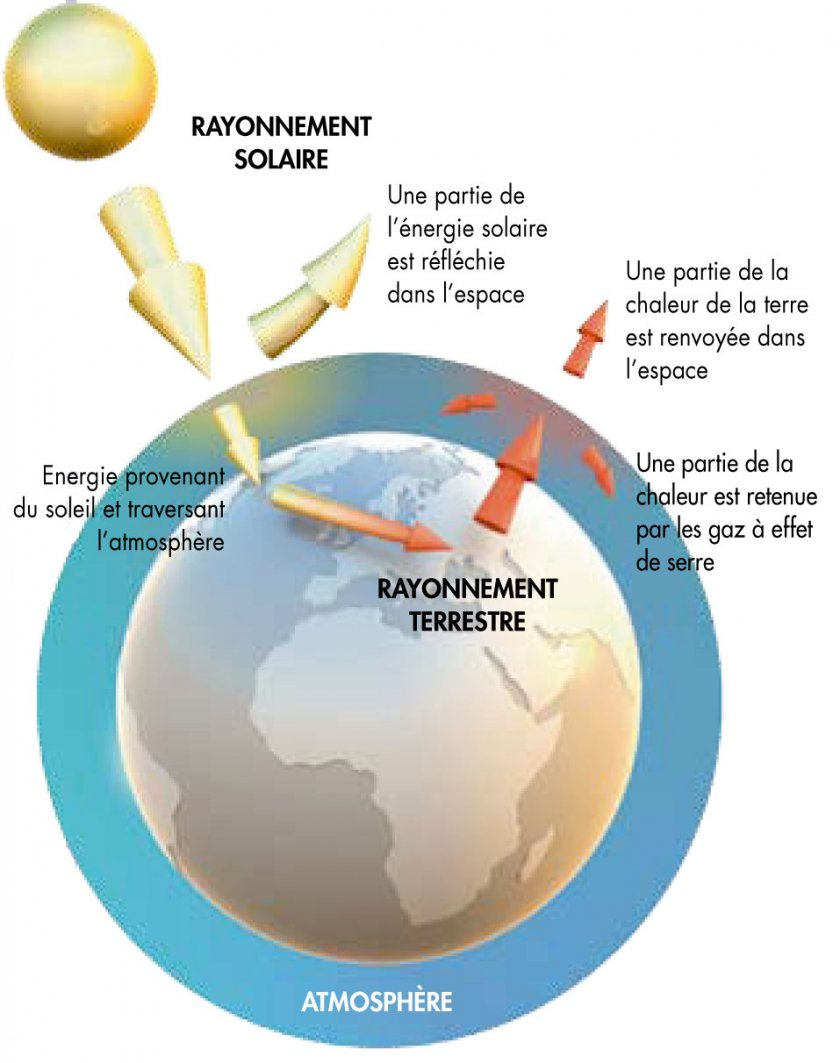
\includegraphics[scale=0.3]{fig/effet-de-serre}
    \par\end{centering}
  \caption{Schéma explicatif de l'effet de serre}
  \label{fig:effetserre}
\end{figure}


Les  gaz à  effet  de serre  peuvent  être repartis  en  deux groupes,  lesquels
existent naturellement et sont aussi produit dans l'industrie, et les outres que
sont seulement industriel.
Pour le premier groupe on a les principaux gaz à effet de serre suivant:
le vapeur d'eau, le dioxyde de carbone, le méthane,le protoxyde d'azote et l'ozone.
Pour le deuxième groupe on a des gaz fluorés comme :
les hydrochlorofluorocarbures, 
les chlorofluorocarbures, 
le tétrafluorométhane et
l'hexafluorure de soufre.

Le  tableau \ref{tab:gaz}  au dessous  démontre le  changement  de concentration
provoquer par l'homme. On peut voir que le dioxyde de carbone a une augmentation
considérable à cause de les actions anthropiques. 

\begin{table}[H]
  \begin{tabular}{ |c | c| p{3cm} | p{2.5cm} | p{2.5cm}  |}
    \hline
    Gaz à effet de serre & Formule & Concentration Préindustrielle & Concentration
    Actuelle & Durée de séjour
    (ans)  \\
    \hline 
    \hline 
    vapeur d'eau & \ce{H2O} & 3‰ & 3‰ &  (1-2 semaines) \\
    dioxyde de carbone & \ce{CO2} & 278 ppm & 387 ppm &  15 - 200 \\
    méthane & \ce{CH4} &0,7 ppm &1,7 ppm& 4 \\
    protoxyde d'azote & \ce{N2O} & 0,275 ppm &0,311 ppm &120 \\
    dichlorodifluorométhane  & \ce{CCl2F2} & 0 & 0,503 ppb & 130 \\
    chlorodifluorométhane  & \ce{CHClF2} & 0 & 0,105 ppb & 12 \\
    tétrafluorométhane & \ce{CF4} & 0& 0,070 ppb &50 000 \\
    hexafluorure de soufre & \ce{SF6} & 0 & 0,032 ppb & 3200\\
    \hline
  \end{tabular}
  \label{tab:gaz}
\end{table}

Le  tableau ci-dessous  montre le  valeur de  Potentiel de  réchauffement global
(PRG), qu'est utilisé pour prédire les impacts relatifs de différents gaz sur le
réchauffement global en se basant sur leurs propriétés radiatives.
Par définition,  le PRG du  \ce{CO2} est  toujours identique à  1 et les  autres sont
basées sur une comparaison avec le \ce{CO2}.

\begin{table}[H]
  \begin{center}
    \begin{tabular}{ |c | c|}
      \hline
      gaz à effet de serre &  PRG à 100 ans \\
      \hline 
      \hline 
      vapeur d'eau &  8\\
      dioxyde de carbone  & 1\\
      méthane & 23\\
      protoxyde d'azote  &310\\
      dichlorodifluorométhane  & 6 200 - 7 100\\
      chlorodifluorométhane  & 1 300 - 1 400\\
      tétrafluorométhane &6 500\\
      hexafluorure de soufre & 22 800\\
      \hline
    \end{tabular}

  \end{center}
\end{table}

Les actions qui on résulté en cette augmentation sont:

\begin{itemize}

\item L'utilisation massive de combustibles fossiles (le charbon, les produits
  pétroliers et le gaz naturel)

\item La  déforestation, parque une forêt  mature est un  réservoir important de
  carbone.

\item  Les  rejets  de  méthane non naturels  sont  dus  principalement  aux
  ruminants et aux surfaces inondées telles les rizières.

\end{itemize}



\subsection{L’impact et le danger liés au réchauffement climatique}

Le principal  impact lié  au réchauffement climatique  est l'augmentation  de la
température, dans la dernière décennie  la moyenne était $0.5^{\circ}$ plus haut
que le période entre 1961 et 1990.

Cette  augmentation de température  influence les  précipitations dans  tout le
monde,  dans quelques  lieus il  y aura  une augmentation  de  précipitation que
pourrait cause  une inondation , tandis  qu'autres lieus auront  des périodes de
sécheresse en raison d'une baisse de précipitations.

Une autre conséquence  est la diminution de la banquise,  soit dans le montagnes
(voir figure \ref{fig:kili}) soit dans les pays avec calottes polaires (Antarctique et Groenland).
Comme quelques montagnes sont la source de l'eau pour quelques civilisations, le
réchauffement climatique  aura un impact  gigantesque dans la quantité  de l'eau
disponible. Et en plus, il existe un danger de avalanche plus accentué.

\begin{figure}[H]
  \begin{centering}
    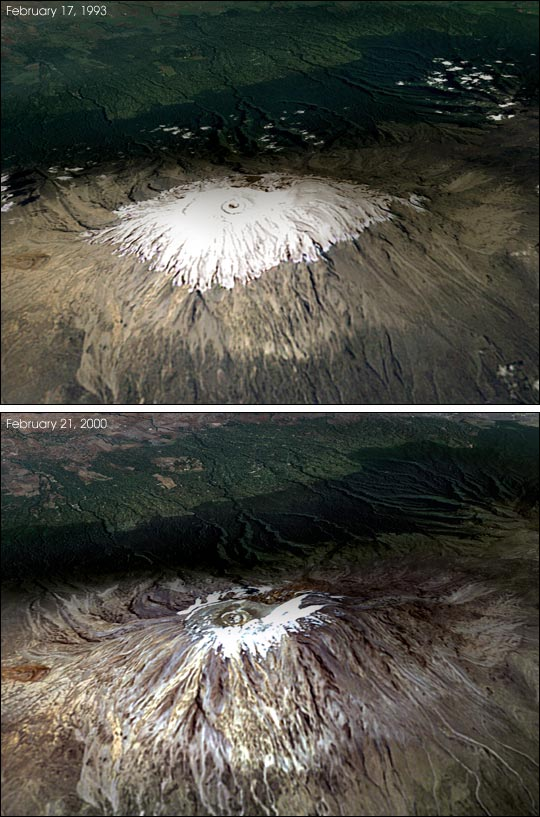
\includegraphics[scale=0.3]{fig/kili}
    \par\end{centering}
  \caption{Changement de l'accumulation des neiges au sommet du Kilimandjaro}
  \label{fig:kili}
\end{figure}


Sur  l'agriculture, les  températures  ont un  effet  sur la  date des  récoltes
agricoles, par exemple les dates de vendanges peuvent être plus avancées que le normal.

Un  changement du  climat, aura  aussi une  impact sur  le faune  et  flore, par
exemple quelques espèces à cause de  la glace fondante doivent se déplace, ainsi
comme les  du mer  qui à causse  d'une augmentation  de température de  l'eau se
déplacement pour le pôles.

D'autres danger sont:
\begin{itemize}
\item L'intensité des cyclones tropicaux va probablement augmenter.
\item Élévation  du niveau de la  mer: le niveau  a augmenté 1,8mm par  an entre
  1961 et 1993 et de 3,4 mm par an depuis 1993. Cette augmentation du niveau est
  en raison de la dilatation thermique des océans et la fonte des glaces continentales.
\end{itemize}


\subsection{Les conséquences en France}


Le réchauffement constaté en France métropolitaine au cours du $XX^e$ siècle 
est d’environ 30  \% plus grand que le réchauffement moyen  sur le globe, tandis
que  la température  moyenne annuelle  global a  augmenté de  $0,74^{\circ}C$ en
France métropolitaine la valeur est de $0,95^{\circ}C$ (voir figure \ref{fig:franceMoyenne}).
En raison de ce réchauffement, on a une augmentation des précipitations
pendant l'hiver et l'automne (entre 5 et 35 \%) et d’une baisse des précipitations
pendant l'été.

Comme prévision dans le cas plus pessimiste,  la moyenne ira augmenter environ $8,0^{\circ}C$ et
dans le cas plus optimiste $3,0^{\circ}C$.

\begin{figure}[H]
  \begin{centering}
    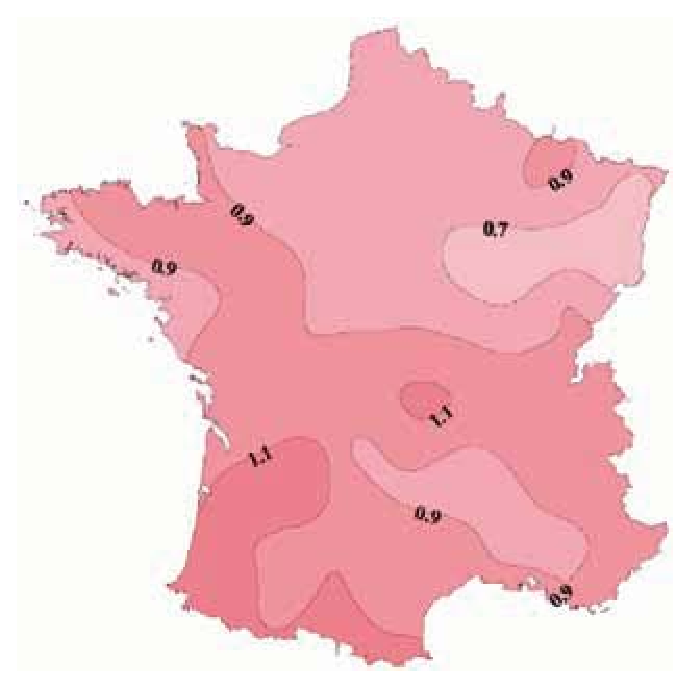
\includegraphics[scale=0.6]{fig/franceMoyenne}
    \par\end{centering}
  \caption{Augmentation de la température moyenne annuelle en France
métropolitaine sur la période 1901-2000}
  \label{fig:franceMoyenne}
\end{figure}

Il  existera aussi  plus  de  jours avec  températures  maximales supérieures  à
$35^{\circ}C$ en  France, la  figure \ref{fig:35france} démontre  les prévisions
qui ont été  faites. Dans la situation plus pessimiste  la France souffrira plus
de cinquante jours avec de grande températures. 

\begin{figure}[H]
  \begin{centering}
    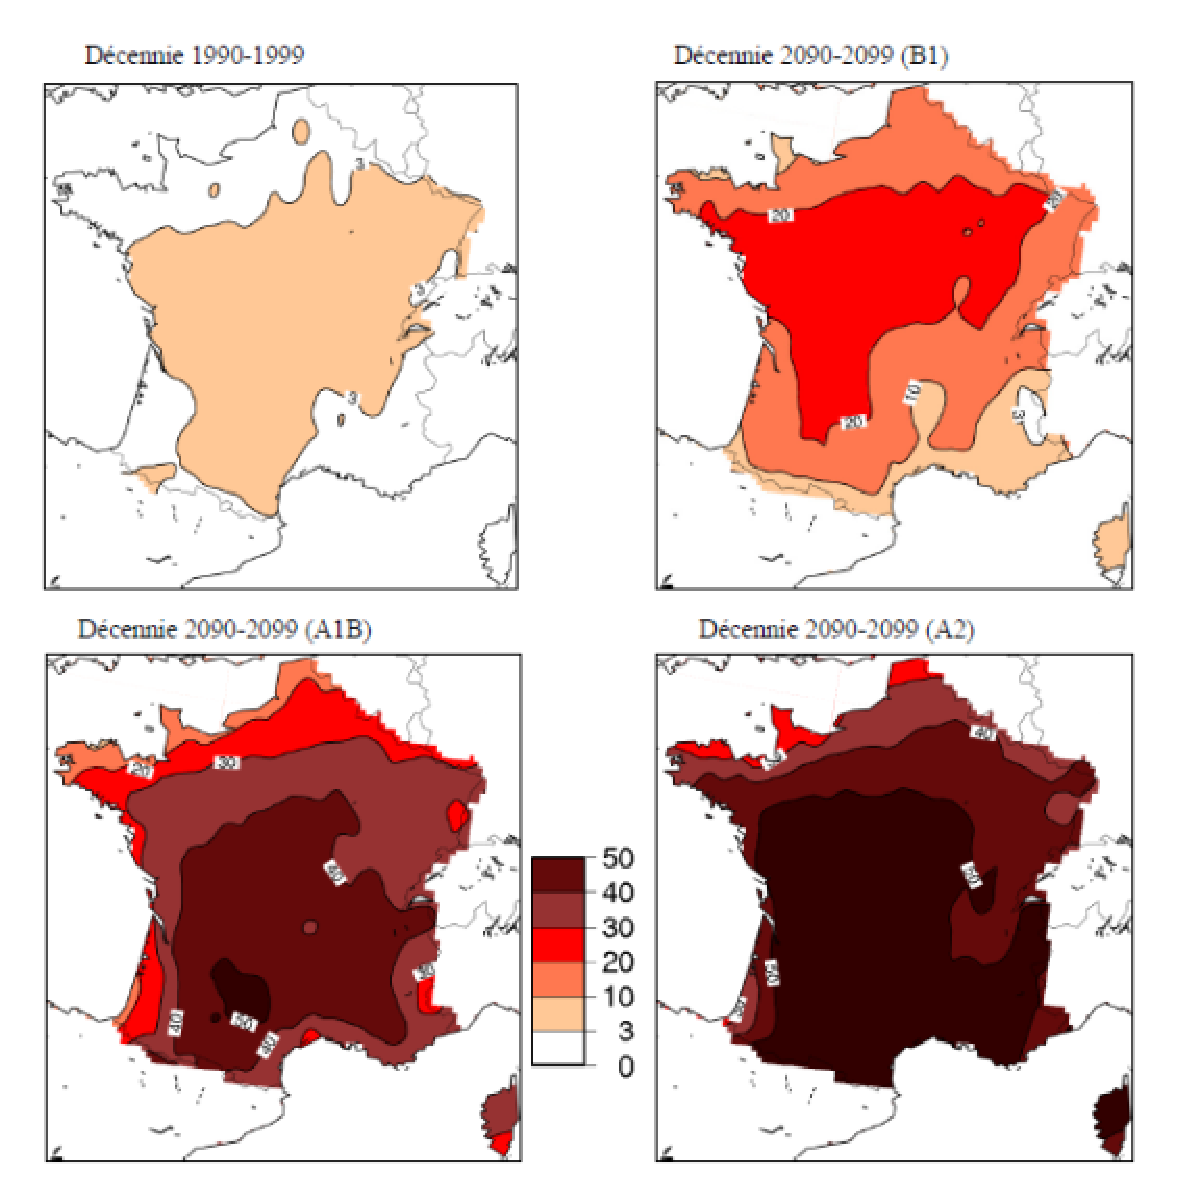
\includegraphics[scale=0.6]{fig/35france}
    \par\end{centering}
  \caption{Nombre de jours par an avec températures maximales supérieures à 35°C en France : dernière décennie du 20 ème siècle comparée à la dernière décennie du 21ème siècle, selon les 3 scénarios A2, A1B et B1 (copyright Météo-France 2007)}
  \label{fig:35france}
\end{figure}


Ressource en eau
Si l’on considère une stabilité de la demande, un déficit de 2 milliards de m3
par an pour la satisfaction des besoins actuels de l’industrie, l’agriculture (irrigation) et l’alimentation en eau potable serait observé à l’horizon 2050

Impact sur la couverture neigeuse
Comme la couverture neigeuse des massifs montagneux français sont liées a bas températures, le réchauffement climatique tend à diminuer la durée de l’enneigement et l’épaisseur du manteau neigeux. De même façon il existera  des modifications des régimes hydrologiques des rivières de montagne, de la végétation à haute altitude et de l’enneigement des stations de sport d’hiver. 

Impact sur l’agriculture
Dans une côté, le sud de la France  devraient apparaître des effets négatifs, qui peuvent prendre une grande ampleur dans le cas de sécheresses répétées et persistante. Dans autre côté, des effets plutôt positifs sont à attendre dans le nord parce que les mauvaises herbes seront les plus impactées.


\section{La position de la société française}
\subsection{Les écologistes}
\subsection{La société en général} 
\subsection{Les entreprises}
\subsection{Les économistes} 


\section{L’avis du gouvernement}
\subsection{Les politiciens}
\subsection{Les lois et taxes}
\subsection{Les traités internationaux}


\section{Analyse des solutions proposés par chaque partie}
\subsection{Présentation des solutions}
\subsection{Comparaison des solutions et son impact dans la société}


\section*{Conclusion}
\section*{Bibliographie}

\end{document}